\documentclass[11pt]{ctexbeamer}

\usetheme{Madrid}
\usecolortheme{default}
\setbeamertemplate{caption}[numbered]
\setbeamertemplate{navigation symbols}{}
\setbeamertemplate{itemize item}[triangle]
\setbeamertemplate{itemize subitem}[circle]

\usepackage{booktabs}
\setCJKmainfont{AR PL SungtiL GB}
\setCJKsansfont{AR PL KaitiM GB}

\title{自监督预训练可以提高DQN样本效率吗}
\author{陈嘉诚 \quad 张礼贤 \quad 刘一非 \quad 谭泽宇}
\date{\today}
\institute{深圳河套学院}

\begin{document}

% ===== 1. Title =====
\begin{frame}
\titlepage
\end{frame}

% ===== 2. Motivation & Problem =====
\begin{frame}{研究背景与问题}
\begin{block}{核心矛盾}
现实中 RL Agent \textbf{看不到真实状态}，只能通过高维传感器观测，导致\textbf{样本效率急剧下降}。
\end{block}

\begin{block}{研究问题}
\begin{enumerate}
\item 观测维度 $M$ 如何影响 DQN 样本效率？
\item 自监督预训练（SSL）能否缓解维度灾难？
\end{enumerate}
\end{block}

\vspace{0.2cm}
\small
\textbf{方法}：可控 8×8 GridWorld $\;\to\;$ MLP 模拟不可逆传感器 $\;\to\;$ 系统比较三条管线（SSL→DQN / DQN-only / Identity）
\end{frame}

% ===== 3. Method: Framework =====
\begin{frame}{实验框架：三条管线}
\vspace{-0.3cm}
\begin{center}
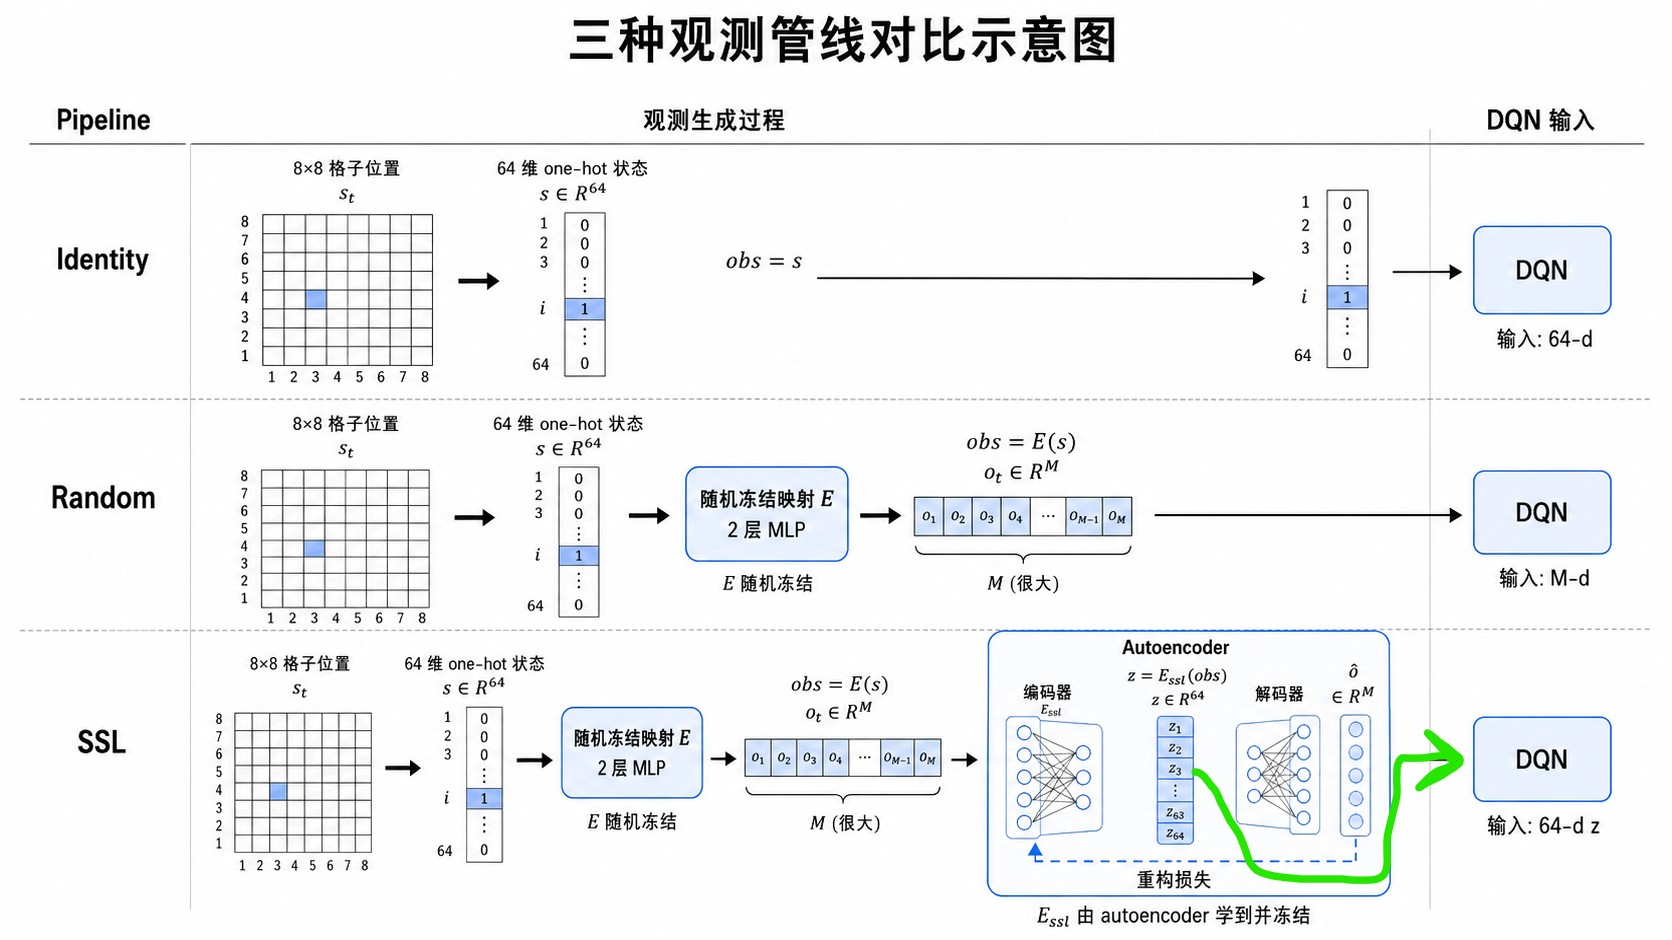
\includegraphics[width=0.9\textwidth]{figure/pipeline.jpg}
\end{center}

\end{frame}

% ===== 6. Results: Table + Efficiency =====
\begin{frame}{核心结果：样本效率}
\begin{columns}[c]
\column{0.45\textwidth}
\small
\begin{tabular}{cccccc}
\toprule
管线 & $M{=}128$ & $M{=}256$ & $M{=}512$ & $M{=}1024$ \\
\midrule
SSL→DQN & 250 & 280 & 180 & \textbf{220} \\
DQN-only & \textbf{160} & 180 & 530 & \textcolor{red}{840} \\
\bottomrule
\multicolumn{5}{c}{Identity: 250 ep, 100\% SR} \\
\end{tabular}
\vspace{0.2cm}

\begin{block}{关键发现}
\begin{itemize}
\item $M{=}1024$：SSL→DQN 是 DQN-only 的 \textbf{3.8×}
\item DQN-only $M{=}1024$ 仅 40\% 最终成功率
\item SSL→DQN 在所有 $M$ 下\textbf{保持稳定}
\item SSL→DQN 在低维度下略逊于 DQN-only （为什么呢）
\end{itemize}
\end{block}

\column{0.55\textwidth}
\vspace{1 cm}
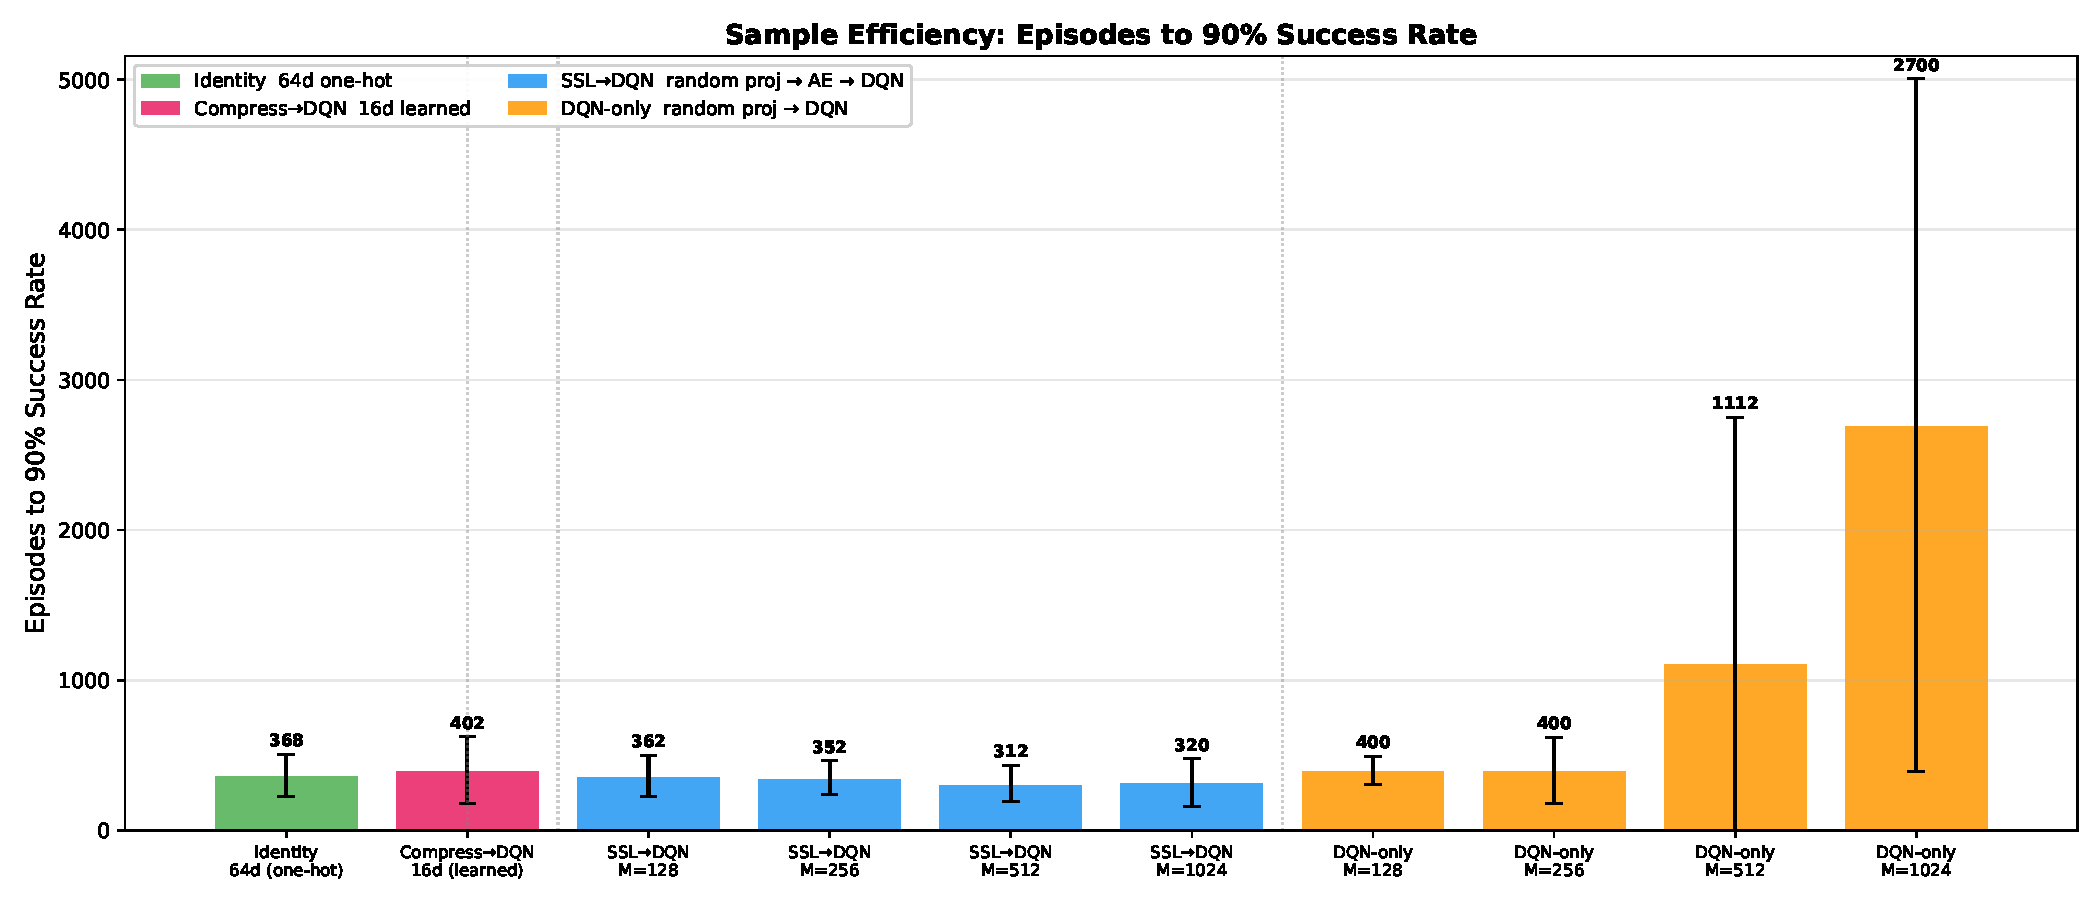
\includegraphics[width=\textwidth]{../analysis_output/sample_efficiency.pdf}
\end{columns}
\end{frame}

% ===== 7. Results: Learning Curves =====
\begin{frame}{学习曲线}
\vspace{-0.2cm}
\begin{center}
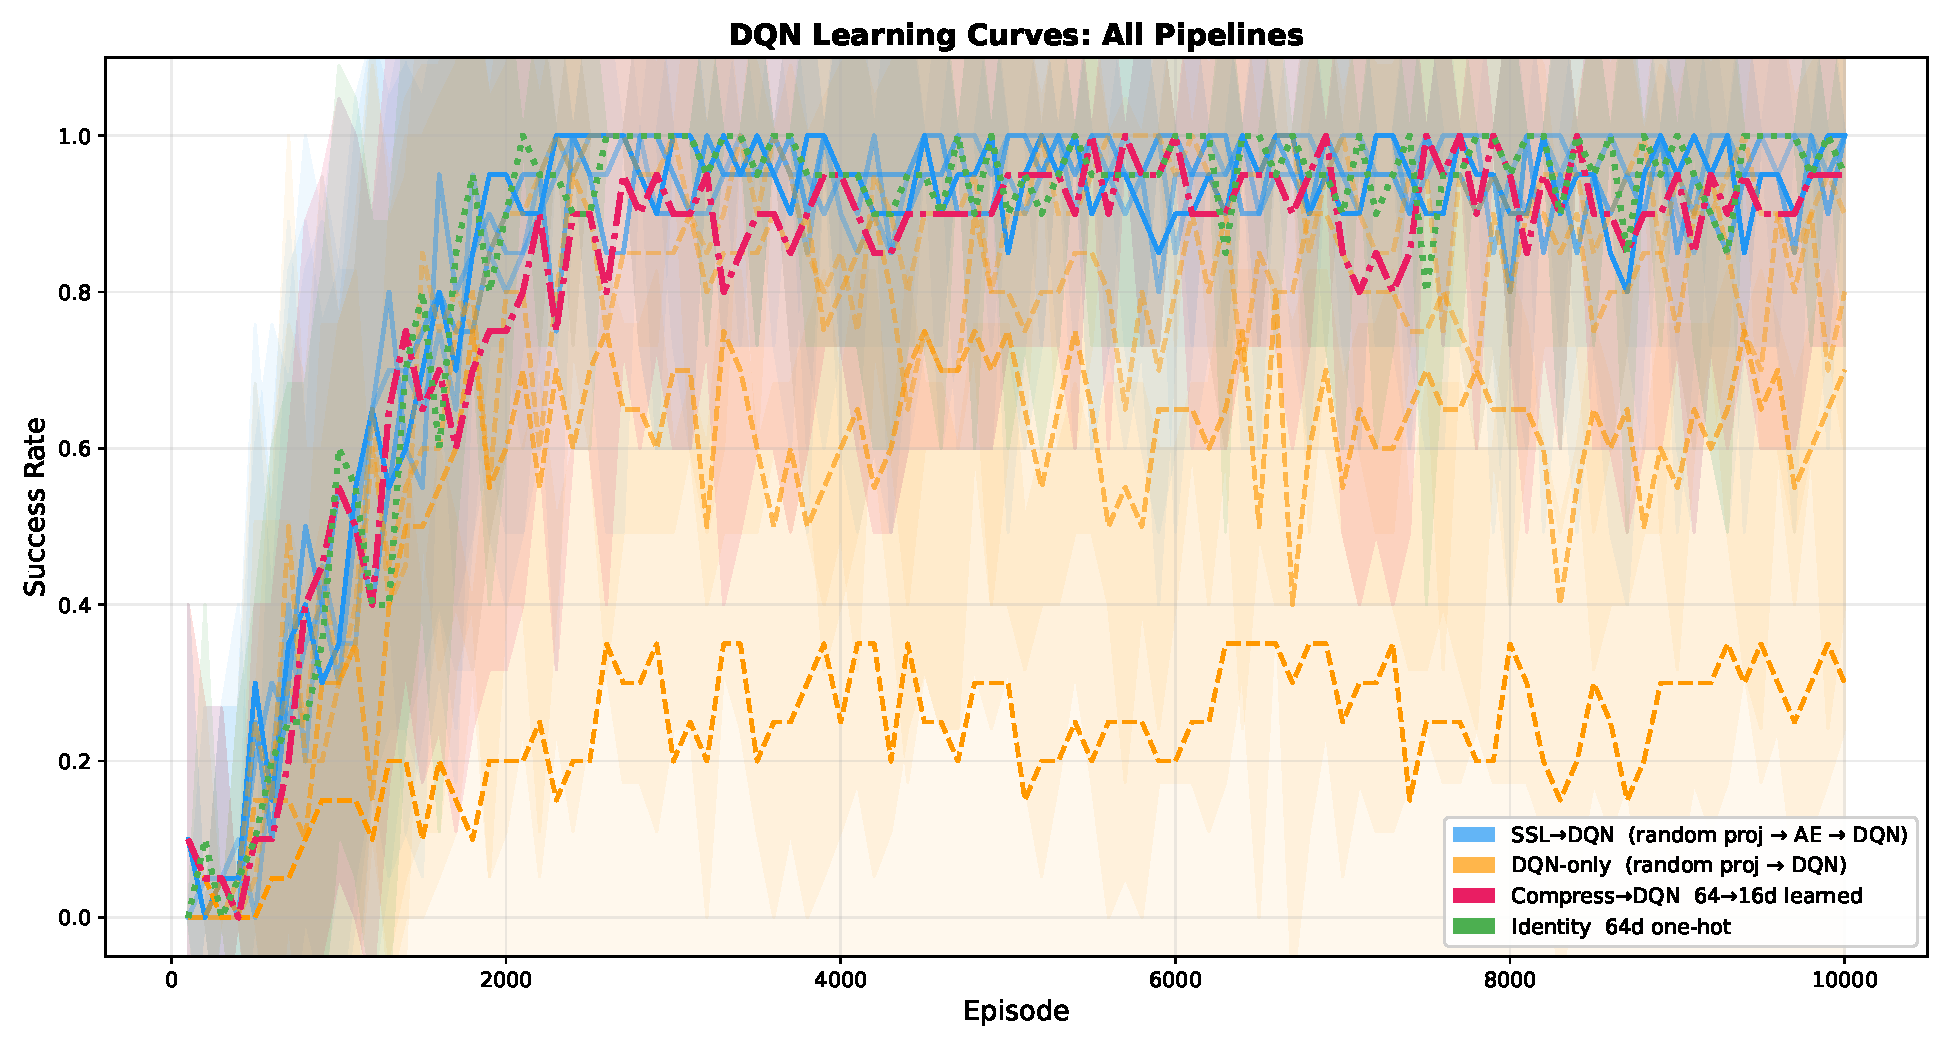
\includegraphics[width=0.75\textwidth]{../analysis_output/learning_curves.pdf}
\end{center}

\vspace{-0.4cm}
\begin{columns}[T]
\column{0.33\textwidth}
\centering\small\textbf{$M{=}128$}\\
DQN-only 最快收敛，SSL 轻微开销
\column{0.33\textwidth}
\centering\small\textbf{$M{=}512$}\\
DQN-only 开始不稳定，方差增大
\column{0.33\textwidth}
\centering\small\textbf{$M{=}1024$}\\
DQN-only 几乎失败，SSL→DQN 稳定保持 100\%
\end{columns}
\end{frame}

% ===== 8. Results: Latent Space =====
\begin{frame}{进一步讨论：潜在维度的可压缩性}
\begin{center}
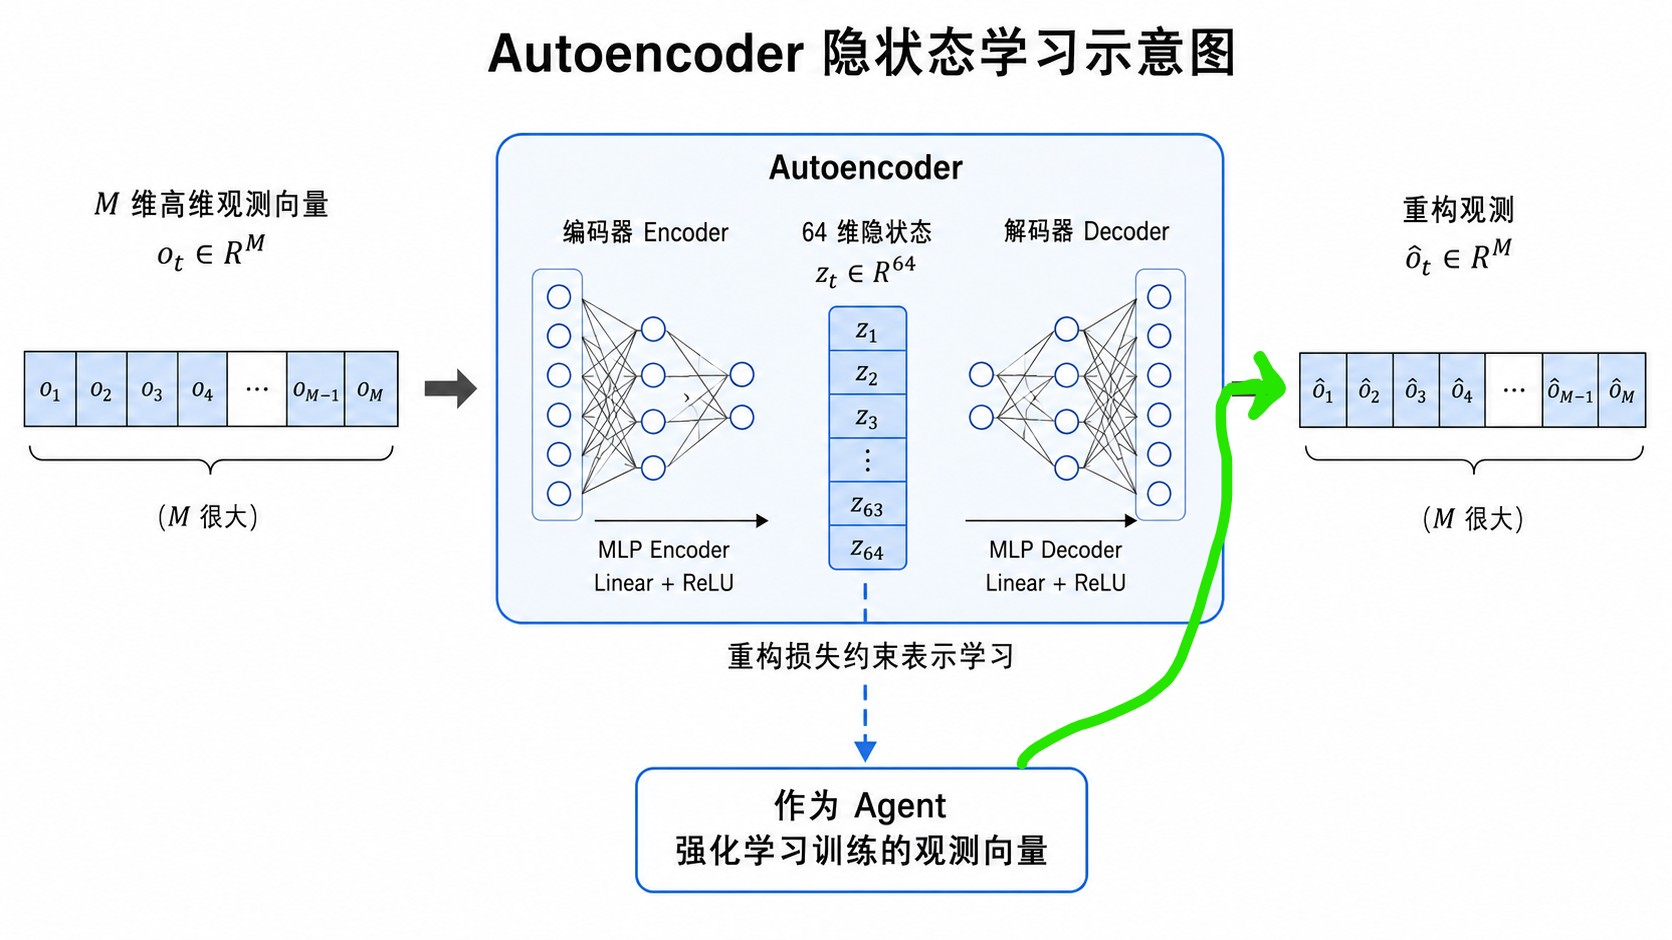
\includegraphics[width=0.55\textwidth]{figure/autoencoder.jpg}

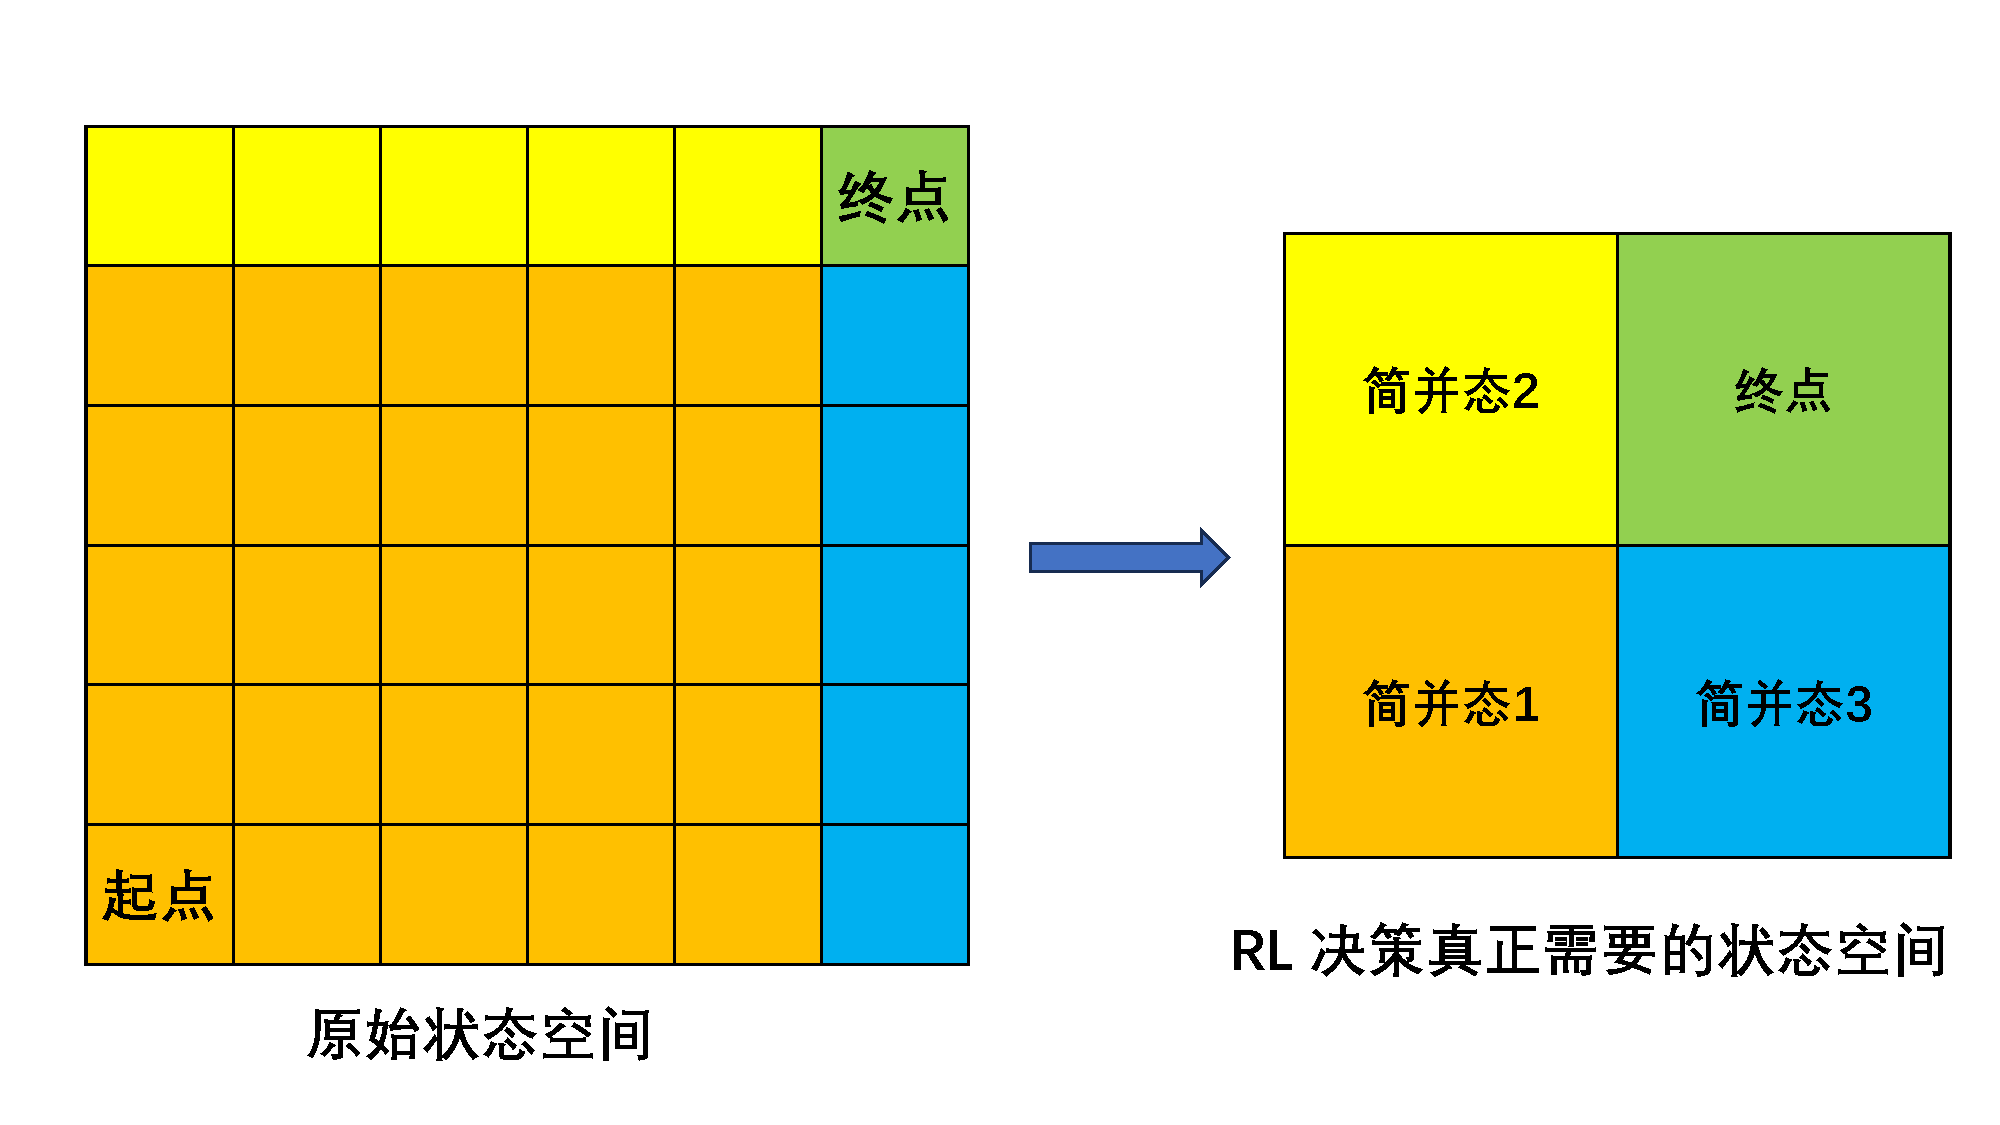
\includegraphics[width=0.55\textwidth]{figure/简并.pdf}
\end{center}
\end{frame}

% ===== 10. Further Discussion =====
\begin{frame}{进一步讨论：潜在维度的可压缩性}
\begin{block}{观察：64 维可能不是下限}
GridWorld 中许多位置存在\textbf{状态简并}。
\vspace{4pt}
\begin{itemize}
\item 例如：棋盘中间大片区域的最优动作都是「向右+向下」组合
\end{itemize}
\end{block}

\begin{block}{SSL 学习到的结构 vs RL 需要的结构}
\begin{itemize}
\item \textbf{Autoencoder} 学的是\textbf{观测重建}：保留 $M$ 维观测的所有变化，包括与任务无关的噪声
\item \textbf{RL 需要}的是\textbf{决策相关}的表示：不同状态只要最优动作相同，就可以映射到同一点
\item 当前 SSL 目标（重建 $\mathbf{o}$）与 RL 目标（最大化回报）存在\textbf{不一致}
\end{itemize}
\end{block}

\begin{alertblock}{核心问题}
如何控制 SSL 的学习目标，使其学到的潜在空间\textbf{对齐 RL 的任务结构}，而非单纯重建观测？\\
这是从「无监督表示学习」走向「任务感知表示学习」的关键一步。
\end{alertblock}
\end{frame}

% ===== 11. Summary =====
\begin{frame}{总结与展望}
\begin{enumerate}
\item \textbf{维度灾难被验证}：DQN-only 在 $M{=}1024$ 时崩溃（40\% SR，44 步路径）
\item \textbf{SSL 有效缓解}：SSL→DQN 保持 100\% SR + 最优路径，与 $M$ 无关
\item \textbf{交叉点存在}：约 $M{\approx}400$ 处 SSL→DQN 超越 DQN-only
\item \textbf{潜在维度可进一步压缩}：RL 状态简并意味着 64 维不是下限，如何让 SSL 学 RL 相关结构是未来方向
\end{enumerate}

\vspace{0.3cm}
\begin{center}
\large \textbf{谢谢！欢迎提问。}
\end{center}
\end{frame}

\end{document}
